\section{圧力のかかった分割リング}
最初の例は、圧力荷重を受けた分割リング(リングの1/4)です。その寸法は:
\begin{itemize}
\item 外径:150 mm
\item 内径:90 mm
\item 厚さ: 20 mm
\end{itemize}
\begin{enumerate}
\item
	{[}mm, ton, s, °C{]}単位の新規ファイルを作成し、ステップ形式のジオメトリをPrePoMaxにインポートします。
	次に、パーツをメッシュ分割します。ここでは、最大要素サイズとして3mmを選択し、その他の設定は変更しませんでした(図\ref{fig:01-01})。
	\begin{figure}[H]
	\centering
	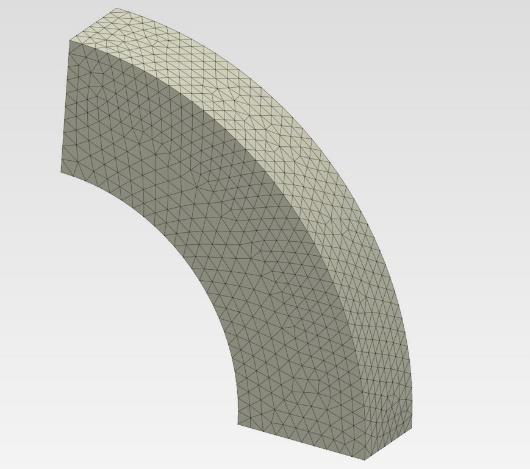
\includegraphics[width=78mm]{fig/01-01.png}
	\caption{分割リング - メッシュ}
	\label{fig:01-01}
	\end{figure}
\item
	境界条件と荷重を適用する際に使用するノードセットfix(下側)とサーフェスpress(上側)を作成します。
\item 
	Steelという名前の新しい材料を定義し、弾性挙動を加え、ヤング率を210000MPa、ポアソン比を0.3と指定します。
	材料にSteelを使用し、Steel\_sectionという名前のソリッドセクションを新規に作成し、そのセクションが割り当てられるように分割リングを選択します。
\item
	デフォルトの設定で静的解析ステップを定義します。
\item
	fixという名前のノードセットに固定境界条件を追加します。
	pressという名前のサーフェスに圧力荷重を追加し、その大きさを20MPaに指定します(図\ref{fig:01-02})。
	\begin{figure}[H]
	\centering
	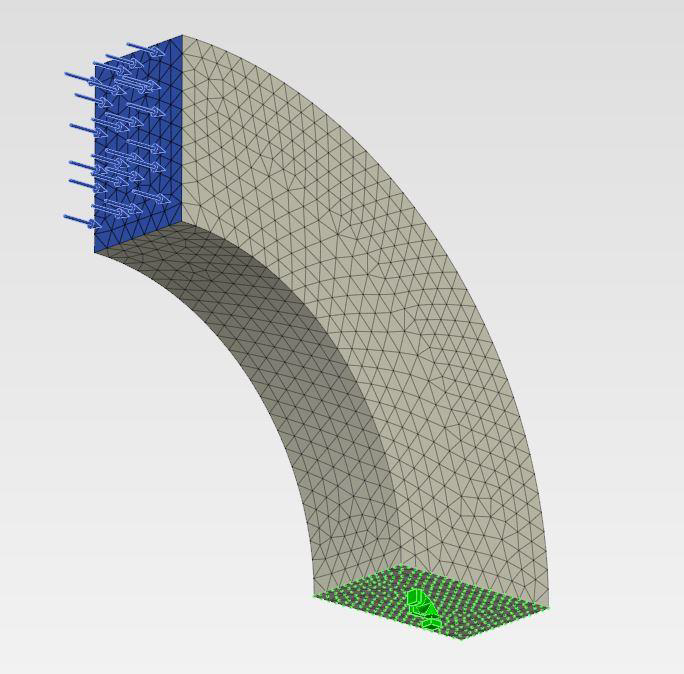
\includegraphics[width=78mm]{fig/01-02.png}
	\caption{分割リング - 境界条件と荷重}
	\label{fig:01-02}
	\end{figure}
\item
  必要な定義がすべて行われたので、解析を提出できます。
  解析が終了するまで待って、結果を開きます。
\item
  ミーゼス応力と変位のコンタープロットを確認します。
  カラースペクトルの種類をRainbowに変更します。
  最大値ラベルを非表示にし、数値フォーマットを一般に変更し、変形スケール係数を40に設定します(図\ref{fig:01-03})。
  分析的に計算された最大応力値は230.68MPaであり、固定面の外側短辺を確認した場合のシミュレーション結果にも同様の応力が見られます。
	\begin{figure}[H]
	\centering
	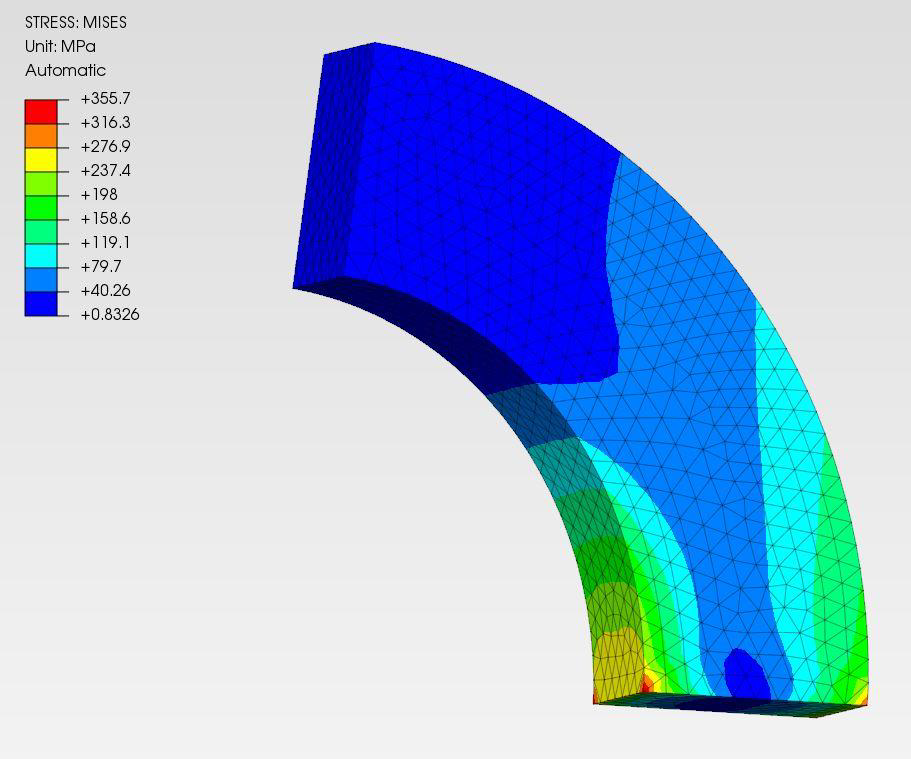
\includegraphics[width=90mm]{fig/01-03.png}
	\caption{分割リング - フォンミーゼス応力}
	\label{fig:01-03}
	\end{figure}
\end{enumerate}